% !TEX TS-program = LuaLaTeX

\documentclass{coderdojo}

\usepackage[lf,sfdefault]{gandhi}

\def\SRC{../pygame/Coding_Games_in_Python__DK__2018.pdf}
\def\MUcode{/Users/kmurphy/mu_code/coderdojo_tramore/fruit_ninja_games/}

\newfontfamily{\pygameZeroFont}{Marker Felt}
\def\pygameZero{{\pygameZeroFont Pygame Zero}}
\def\MuEditor{{\pygameZeroFont Mu}}

\usepackage{pdflscape}

\usetikzlibrary{decorations,decorations.pathreplacing,decorations.pathmorphing}
\tikzstyle{postit}=[fill=yellow!50,draw,thick,
decorate, drop shadow,
decoration={random steps,segment length=3pt,amplitude=1pt},
text width=4cm, font=\scriptsize]

\worksheet{20}{Python --- CoderDojo Tramore}

\newcommand\contentsitem[2]{
	\item \hyperref[#1]{\color{section}\bfseries #2}
}

\usepackage{wrapfig}
\usepackage{float}

\newcommand\TODO[1]{
\begin{itemize}
\item[\todoSymbol] \color{todo} #1
\end{itemize}}


\newcommand\TEST[1][\bf Test your code!]{
	\centerline{\tikz\node[starburst, fill=yellow, draw=red, line width=2pt,align=center] {#1};}
}

\newcommand\TESTSMALL[2][\bf Test your code!]{
{\tikz[scale=#2]\node[starburst, fill=yellow, draw=red, line width=2pt,align=center] {#1};}
}

\usetikzlibrary{decorations.pathreplacing}

%: DOCUMENT
\begin{document}
\maketitle

\section*{Introduction}

It is January 2020! A new year is a good time to review what tools we use to develop our python code and which python modules we use. For the last few years we have used:
\begin{itemize}
\item 
Python editor \href{https://thonny.org}{Thonny (thonny.org)}. This is a nice editor and has lots of features for people starting to code in python. However, I want to try out a new editor to see if it suits our needs more.
\item
Python module \code{turtle} to generate graphics.  As you have seen, this module allow us to create many turtles, each of which, can be given instructions to move and draw out shapes.  I  like this module and we (or you) have done some cool stuff using it. But it is not so great at writing games with fancy graphics (animations) and sound. So let's try something new.

\end{itemize}

\begin{figure}[H]\centering
\begin{tikzpicture}
\node (P) {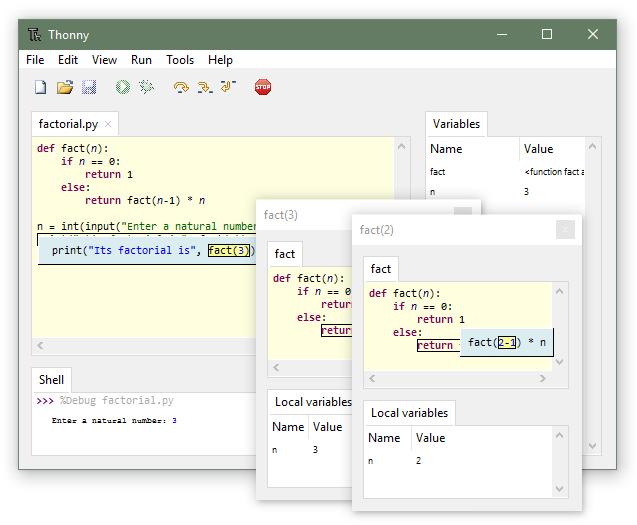
\includegraphics[height=3cm]{Thonny}};

\foreach \x/\y/\a/\l in {
	2/0.7/10/faces, 5.5/0.7/5/batman, 8.5/0.6/-5/chess,11.5/0.6/-5/Completed_Game.png,
	4/-0.7/-10/spiral,7/-0.7/10/city, 10/-0.7/-7/snowman_final} 
	{
	\node[anchor=west,fill=white,drop shadow,rotate=\a] 
	at ($(P.east)+(\x,\y)$)
	{\includegraphics[height=2cm]{\l}};
}

\end{tikzpicture}
\caption{Screenshot of Thonny editor and some sample {\tt turtle} applications (that you have created).} 
\end{figure}

\section{The Future is \ldots\ \MuEditor\ \ldots\ and \ldots\ \pygameZero}

So, our new tool set consists of:
\begin{itemize}
\item Python editor \code{mu-edit}\hfill\href{https://codewith.mu}{codewith.mu}
\item Python game (graphic+sound) module \pygameZero\hfill
\href{https://pygame-zero.readthedocs.io/en/stable/}{pygame-zero.readthedocs.io}
\end{itemize}
and websites for resources (also known as game assets)
\begin{itemize}
\item Game sound effects \hfill\href{https://www.zapsplat.com}{www.zapsplat.com}
\item Background music \hfill\href{https://www.melodyloops.com/music/}{www.melodyloops.com/music}
\end{itemize}
and supporting software 
\begin{itemize}
\item Editing and converting audio files \hfill\href{https://www.audacityteam.org}{www.audacityteam.org}
\item Editing and generating art \hfill\href{https://krita.org/en/}{krita.org/en}
\end{itemize}

% TODO -- add page describing content of USB stick 
% 
%\clearpage
%
%
%\section{The mu-editor}
%
%\centerline{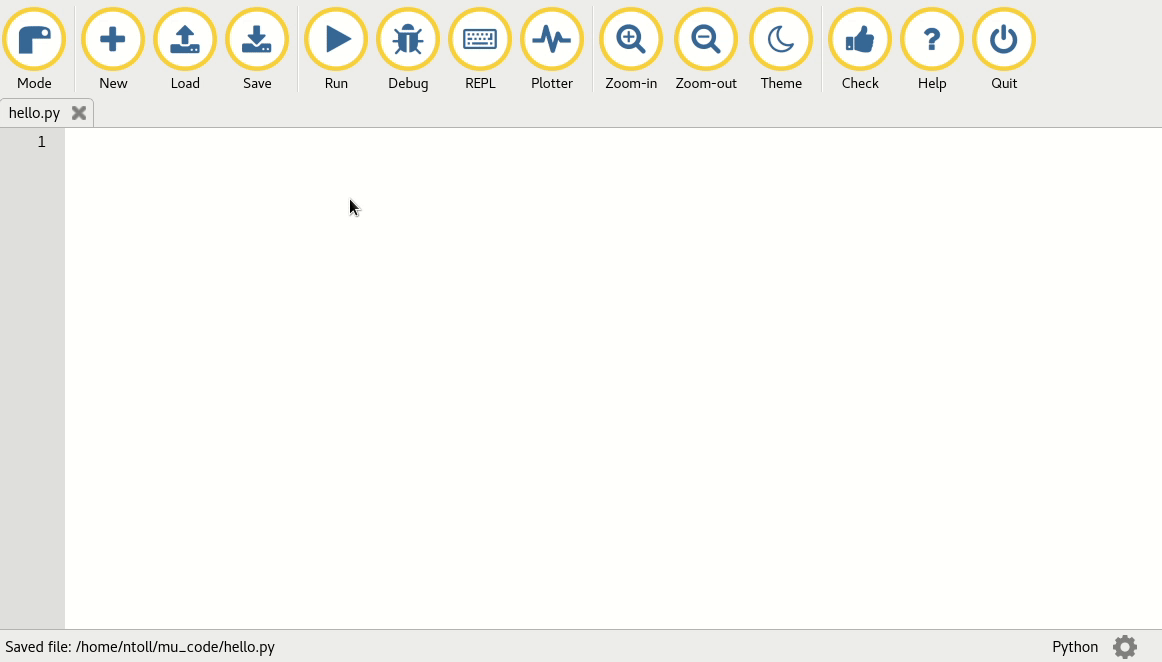
\includegraphics[width=.8\textwidth]{mu-0}}


%: END
\end{document}
